
\documentclass{AbstractTemplate}

\usepackage{graphicx}
\usepackage{epstopdf}

\title{HINT-BC -- HMM-based Identification of Transcription Factor Footprints on Bias-Corrected DNase-seq Data}

\author{Eduardo G. Gusmao\,\affref{ref1}$^{,}$\affref{ref2}$^{,\dag}$, Martin Zenke\,\affref{ref2} and Ivan G. Costa\,\affref{ref1}$^{,}$\affref{ref2}$^{,}$\affref{ref3}$^{,*}$}

\affiliation{
  \aff{ref1}
  	{\footnotesize {IZKF Computational Biology Research Group, RWTH Aachen University Medical School, Aachen, Germany.}}
  \aff{ref2}
  	{\footnotesize {Department of Cell Biology, Institute of Biomedical Engineering, RWTH Aachen University Medical School, Aachen, Germany.}}
  \aff{ref3}
  	{\footnotesize {Aachen Institute for Advanced Study in Computational Engineering Science (AICES), RWTH Aachen University, Germany.}}
  $^{\dag}$ Presenting author \hspace{2cm} $^{*}$ ivan.costa@rwth-aachen.de
}

%\addtolength{\topmargin}{-0.8cm}
\addtolength{\textheight}{0.4cm}

\begin{document}

\maketitle

\section{Introduction}
\label{sec:introduction}

Advances on next-generation sequencing techniques have enabled investigators to develop high-throughput versions of many essays such as chromatin immunoprecipitation (ChIP-seq) and DNase I footprinting (DNase-seq). The latter, a technique in which digested chromatin fragments are sequenced to identify accessible regulatory regions, can be used to accurately identify transcription factor (TF) binding sites through a well-characterized pattern of DNase I cleavage~\cite{crawford2006b,hesselberth2009,neph2012a,encode2012}. In general, transcription factor binding sites (TFBSs) present high levels of DNase I cleavage activity at their flaking regions and low cleavage activity at the positions where proteins are bound (footprints)~\cite{boyle2011}. Recently, many computational footprinting methods have been developed to automatically detect TFBSs based on DNase-seq data~\cite{boyle2011,pique2011,cuellar2012,neph2012a,gusmao2014}.

Nevertheless, it is known that DNase-seq exhibits an intrinsic DNase I cleavage bias~\cite{he2014,meyer2014}. Such bias reflects the binding preference of the DNase I enzyme to certain $k$-mers. Since TFs present binding affinity towards certain DNA sequences, footprints are likely to be affected by DNase-seq cleavage bias. Previous attempts to correct such bias did not result in significant performance improvement~\cite{hesselberth2009}.

Here, we couple a DNase-seq cleavage bias correction strategy with our previous approach, termed HINT (HMM-based identification of transcription factor footprints)~\cite{gusmao2014}. We compare our novel method -- HINT bias-corrected (HINT-BC) -- with seven recent computational footprinting methods in the literature and with its uncorrected version. We study whether bias was mitigated, the impact on computational footprinting performance and the nucleotide-level changes on DNase-seq profile shape for many transcription factors.

\section{Method}
\label{sec:method}

We performed a modified $k$-mer-based bias-correction strategy as presented in~\cite{he2014}. Briefly, the DNase-seq cleavage bias is estimated from the aligned reads inside DNase hypersensitivity sites (DHSs). The observed cleavage score for a particular $k$-mer $w$ is defined as the number of cleavages that occurred centered on $w$. The background cleavage score equals the number of times $w$ occurs. The bias estimation for $w$ corresponds to the ratio between the observed and background cleavage scores. Finally, the bias-corrected DNase-seq signal was created based on the original DNase-seq signal and smoothed versions of the DNase-seq signal and the estimated bias signal.

In this analysis we considered six competing methods: Boyle~\cite{boyle2011}, Neph~\cite{neph2012a}, Centipede~\cite{pique2011}, Cuellar~\cite{cuellar2012}, ranking of TFBSs based on the total number of surrounding DNase-seq reads (referred to as tag-count; TC) and footprint score (FS)~\cite{he2014}. Furthermore, we used the position weight matrix (PWM) motif matching bit-score as a `control' scoring. We compared these methods with HINT~\cite{gusmao2014} and the HINT bias corrected (HINT-BC) version. This comprehensive comparison totals nine methods.

We used DNase-seq aligned reads from ENCODE~\cite{encode2012} (Crawford lab) cell types H1-hESC and K562. To create the validation data set we obtained ChIP-seq enriched regions (peaks) from ENCODE Analysis Working Group (AWG) track and PWMs from Jaspar, Uniprobe and Transfac repositories. The validation data set consists of all putative binding sites obtained by matching the PWMs on the genome. These putative binding sites are considered true TFBSs if they have ChIP-seq evidence and false TFBSs otherwise.

\section{Results}
\label{sec:results}

First we compared the amount of bias with the performance of the methods for K562 cell type. For that, we evaluated the observed {\emph vs.} bias signal (OBS), which can be defined as the Pearson correlation between the average profile of these two signals for all putative binding sites with ChIP-seq evidence. Then, we evaluated the Pearson correlation between the OBS and the area under the ROC curve (AUC) for each TF. We observed that only four out of eight methods (FS, PWM, Boyle and Neph) presented a significant ($p$-value $< 0.05$) negative correlation ($-0.17$, $-0.22$, $-0.3$ and $-0.26$, respectively), i.e. the performance of these methods are being negatively influenced by the DNase-seq cleavage bias. Centipede, Cuellar, HINT and HINT-BC presented a Pearson correlation of $-0.12$, $-0.1$, $-0.05$ and $-0.03$. This is evidence that some computational footprinting methods implicitly correct the bias through signal smoothing. Moreover, the HINT-BC method presented the lowest absolute correlation among all methods, including the non-corrected HINT. This suggests that the bias-correction strategy mitigates the DNase-seq cleavage bias.

Next, we evaluated the performance of the methods with regard to their AUC at the 10\% false positive rate (Fig.~\ref{fig:allresults}A and B). We applied the Friedman-Nemenyi test to compare the AUC values of distinct methods. We observed that methods which are based on segmenting the genome with window-based statistics or HMMs (Boyle, Neph and HINT) outperformed ($p$-value $< 0.05$) methods that classify motif-predicted putative binding sites as bound or unbound (TC, FS, Cuellar, Centipede and PWM) in the specificity level. Also, HINT-BC outperformed all other methods ($p$-value $< 0.05$). Such result demonstrates that a bias-correction strategy improves digital genomic footprinting. However, we point to the fact that some complex approaches such as Centipede and Cuellar are outperformed by the TC method, which does account for nucleotide-level footprint patterns.

The bias correction led to substantial change in the average DNase I cleavage patterns surrounding the TFs. The Fig.~\ref{fig:allresults}C shows examples of such changes for selected TFs in cell type K562. We observed that the bias-corrected DNase-seq signal fits the high affinity regions of the TF motifs. In contrast, uncorrected DNase-seq signal presents a higher signal in the center of the motif, which does not reflect the affinity regions so clearly. Such patterns reflect bias corrections which are beneficial to footprinting method accuracy.

Recently, the performance of computational footprinting techniques was questioned and shown to be outperformed by simple statistics such as ranking putative binding sites based on the number of DNase-seq tag counts within its vicinity~\cite{he2014}. However, we show that our approach successfully address the intrinsic DNase-seq cleavage bias and outperforms a number of competing methods in the literature.

\begin{figure}[h!]
\hspace*{-1cm}
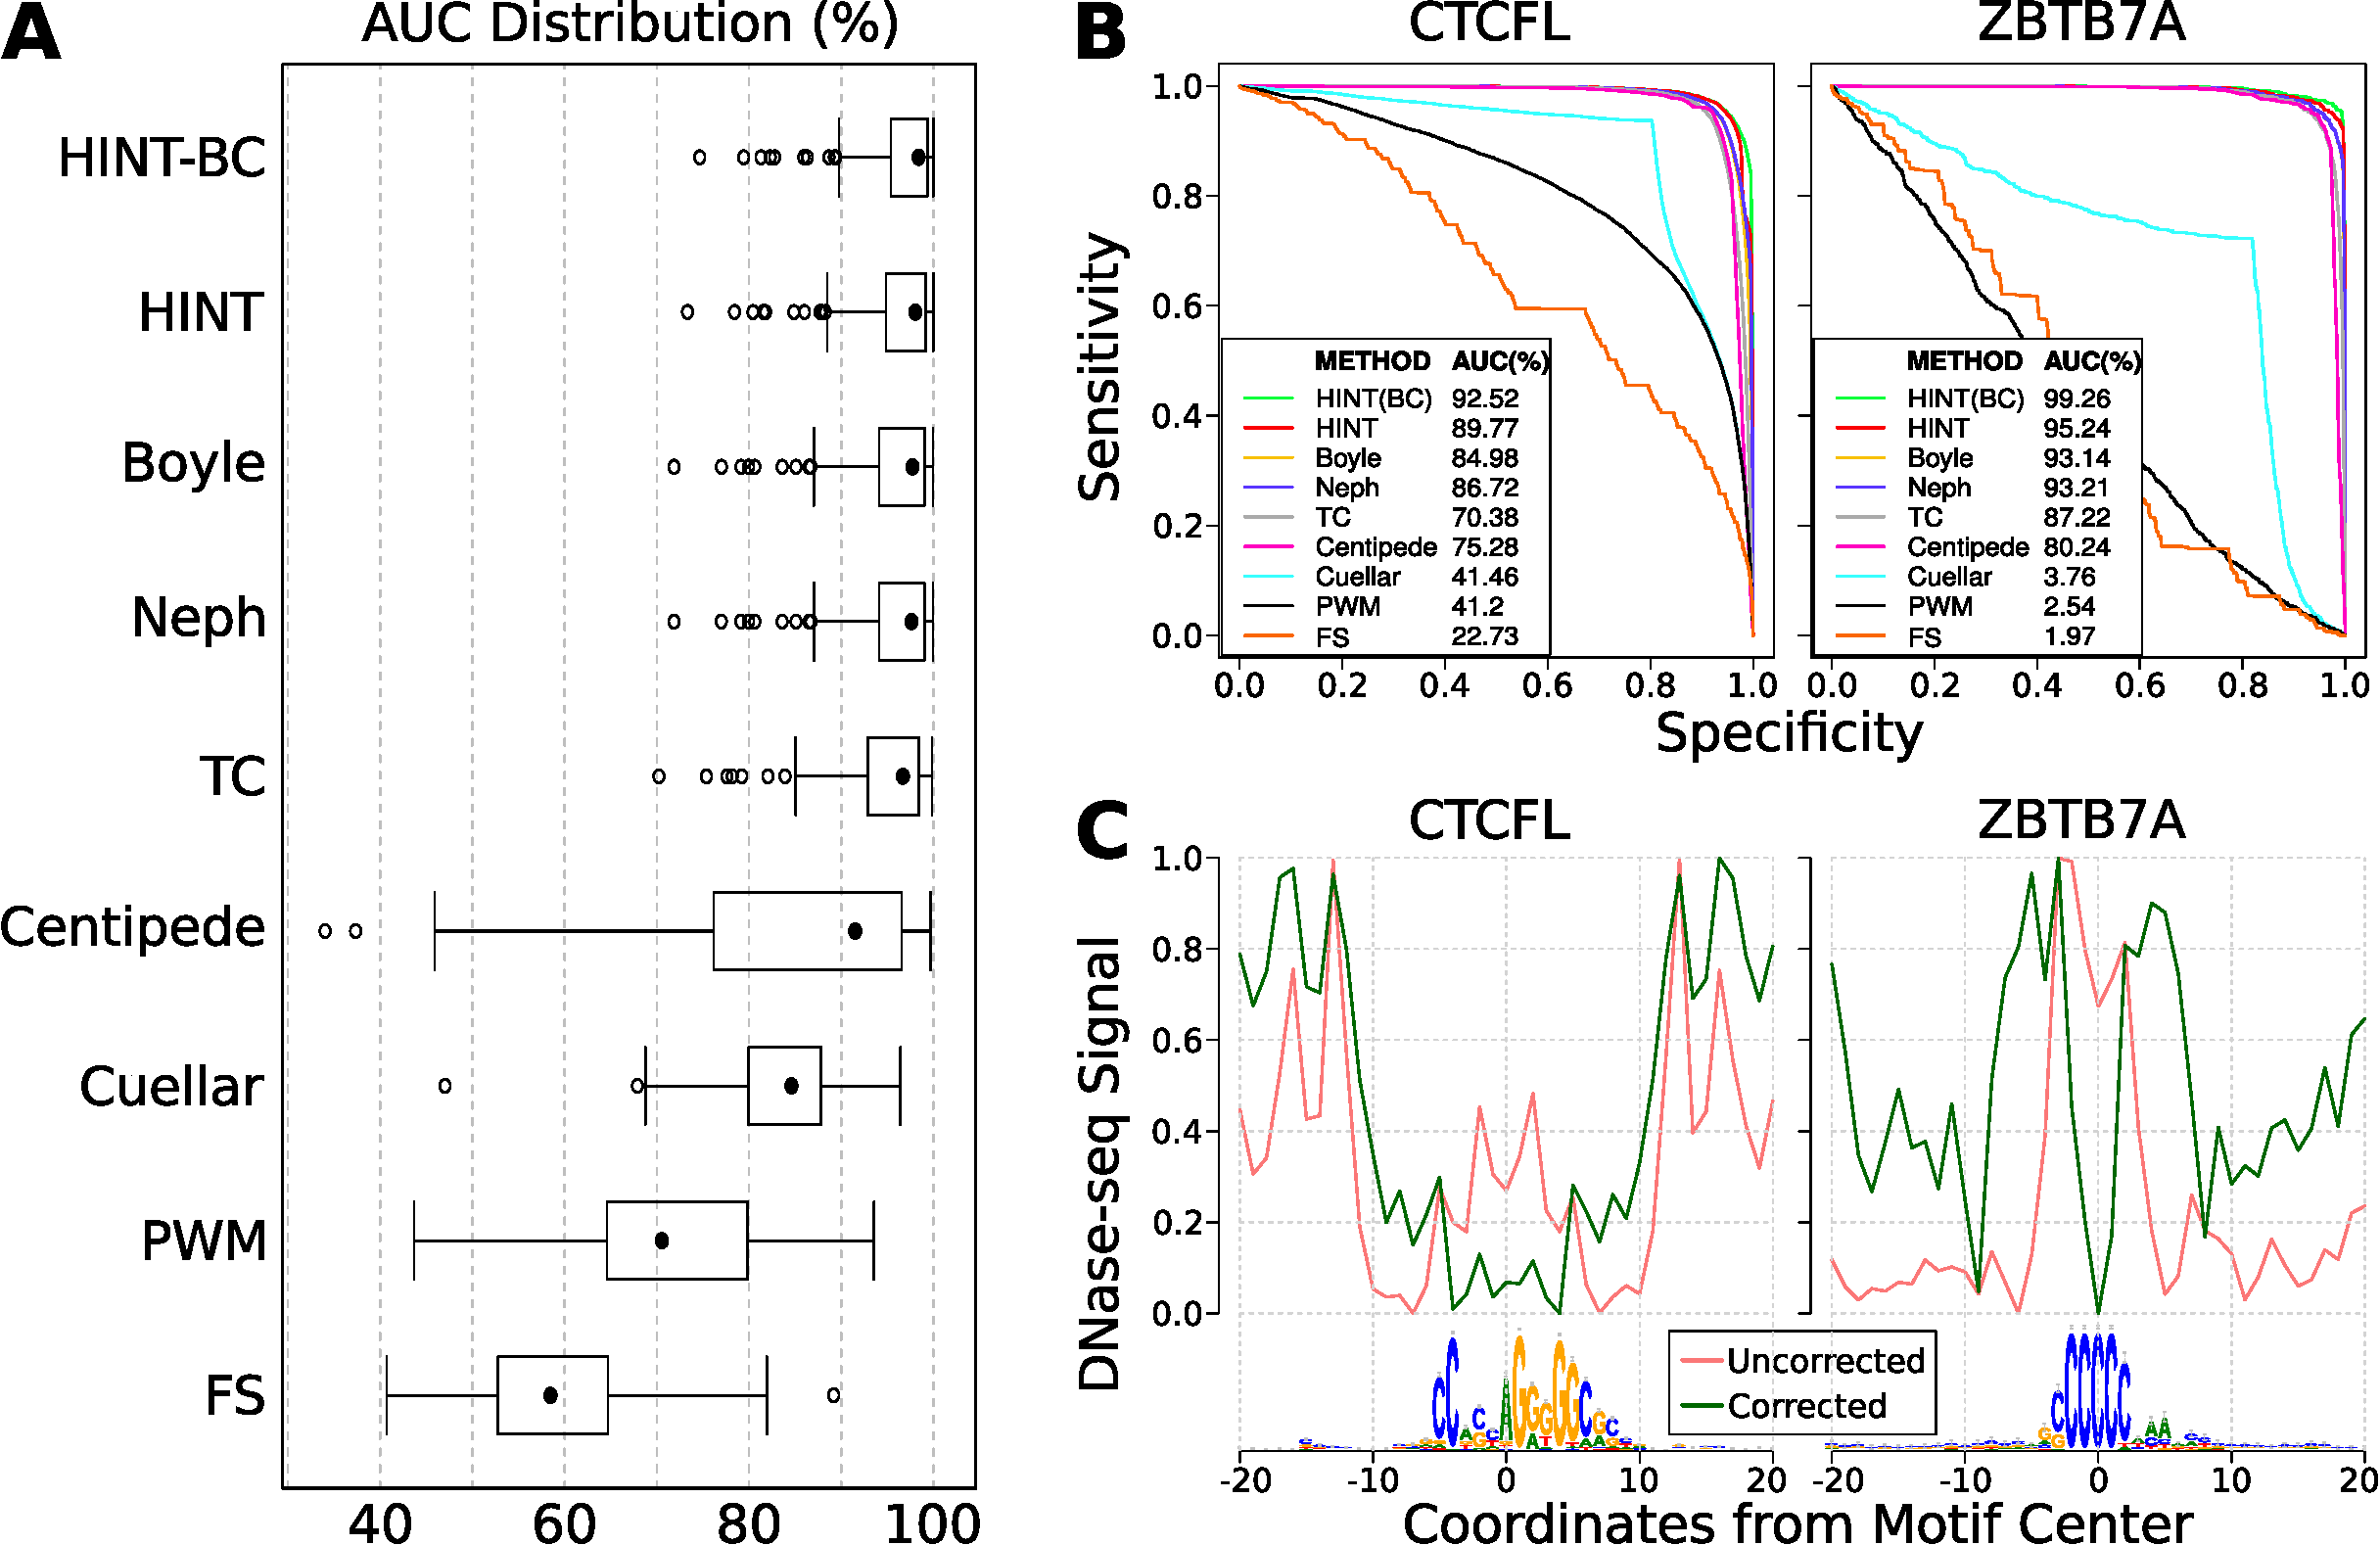
\includegraphics[width=1.1\textwidth]{Figure/Format/Fig_v2.pdf}
\caption{(A) Distribution of AUCs for all methods tested. (B) ROC curves for selected TFs. The AUC at 10\% FPR is shown for all methods. (C) Average uncorrected and bias-corrected DNase-seq signals around selected TFs with ChIP-seq evidence. On the bottom, it is shown the motif logo for all DNA fragments within these regions.}
\label{fig:allresults}
\end{figure}

\paragraph{Funding:}
This work was supported by the Interdisciplinary Center for Clinical Research (IZKF Aachen), RWTH Aachen University Medical School, Aachen, Germany.

\bibliographystyle{AbstractTemplate}
{\footnotesize
\bibliography{document}}

\end{document}
